% Include the per-supervision info file.
\documentclass[10pt,oneside,a4paper]{article}

% Pull in the template, configured as above.
% DO NOT add \usepackage commands here.  Place any custom commands
% into your SV work files.  Anything in the template directory is
% likely to be overwritten!

\usepackage{fancyhdr}

\usepackage{lastpage}       % ``n of m'' page numbering
\usepackage{lscape}         % Makes landscape easier

\usepackage{verbatim}       % Verbatim blocks
\usepackage{listings}       % Source code listings
\usepackage{epsfig}         % Embed encapsulated postscript
\usepackage{array}          % Array environment
\usepackage{qrcode}         % QR codes
\usepackage{enumitem}       % Required by Tom Johnson's exam question header

\usepackage{hhline}         % Horizontal lines in tables
\usepackage{siunitx}        % Correct spacing of units
\usepackage{amsmath}        % American Mathematical Society
\usepackage{amssymb}        % Maths symbols
\usepackage{amsthm}         % Theorems

\usepackage{ifthen}         % Conditional processing in tex

\usepackage[top=3cm,
            bottom=3cm,
            inner=2cm,
            outer=5cm]{geometry}

% PDF metadata + URL formatting
\usepackage[
            pdfauthor={\studentname},
            pdftitle={\svcourse, SV \svnumber},
            pdfsubject={},
            pdfkeywords={9d2547b00aba40b58fa0378774f72ee6},
            pdfproducer={},
            pdfcreator={},
            hidelinks]{hyperref}



\renewcommand{\headrulewidth}{0.4pt}
\renewcommand{\footrulewidth}{0.4pt}
\fancyheadoffset[LO,LE,RO,RE]{0pt} 
\fancyfootoffset[LO,LE,RO,RE]{0pt}
\pagestyle{fancy}
\fancyhead{}
\fancyhead[LO,RE]{{\bfseries Xavier Yeo}\\yhxy2@cam.ac.uk}
\fancyhead[RO,LE]{{\bfseries CST Part II: Quantum Computing}}
\fancyfoot{}
\fancyfoot[RO,LE]{\today\hspace{1cm}\thepage\ / \pageref{LastPage}}
\setlength{\headheight}{22.55pt}

{
  % 2. Right-handed marker, one-sided printing or e-marking, use oneside.
  \setlength{\marginparwidth}{111pt}
}


\setlength{\parindent}{0em}
\addtolength{\parskip}{1ex}


\usepackage{graphicx}
\graphicspath{ {./images/} }

% If you have any additional \usepackage commands, or other
% macros or directives, put them here.  Remember not to edit
% files in the template directory because any changes will
% be overwritten when template updates are issued.

\newcommand{\qb}[1]{\left| #1 \right\rangle}

\begin{document}

% Your work here.
% See example_sv/example.tex for LaTeX examples.

\section*{1. Background}

Qubits are represented by $ \qb{\psi} $, and are defined by 

\[ 
    | \psi \rangle = \alpha | 0 \rangle + \beta | 1 \rangle
\]

where $\alpha, \beta$ are complex numbers such that $|\alpha|^2 + |\beta|^2 = 1$. Here, the probability that the qubit is in the $\qb{0}$ state is given by $|\alpha|^2$ and vice versa for $\qb{1}$. 

Once a qubit has been measured, the system remains in its measured state, and will always yield the same value, unless some quantum operation has been applied to the qubit - fundamentally, only 1 bit of information can be extracted from the qubit. 

It helps to understand that while several values of $\alpha, \beta$ correspond to the same probabilities of $\qb{0}$ and $\qb{1}$, they refer fundamentally to different states, and will evolve differently. We note the following special states: 

\[
    \begin{aligned}
        \qb{+} &= \frac{1}{\sqrt{2}} (\qb{0} + \qb{1}) \\
        \qb{-} &= \frac{1}{\sqrt{2}} (\qb{0} - \qb{1}) \\
        \qb{i} &= \frac{1}{\sqrt{2}} (\qb{0} + i\qb{1}) \\
        \qb{-i} &= \frac{1}{\sqrt{2}} (\qb{0} - i\qb{1}) \\
    \end{aligned}
\]


\section*{2 Linear Algebra}

\subsection*{2.1 Vector Spaces}

Vector spaces need not be vectors. Instead, they can be generalised to the following: A set $V$ is a vector space over $\mathbb{K}$ if: 


\textbf{Addition: } If $u$ and $v$ are elements of $V$ then so is $u + v$. This addition must be associative. 

\textbf{Scaling: } If $u$ is an element of $V$, and $\alpha$ is an element of $\mathbb{K}$, then so is $\alpha u$. This scaling is distributive. 

This gives us a couple of properties: 

\begin{enumerate} 
    \item 
    Other mathematical structures can also be a vector space. For instance, the set of all polynomicals with complex coefficients of degree 2 are vector spaces over $\mathbb{C}$. 

    \item 
    There are also more properties to be checked before deciding if said set is a vector field, but this is often sufficient. 
\end{enumerate}

\subsection*{2.2 Relevance to Quantum Computing}

States of a quanutm system form a vector space and their transformations are described by linear operators. A finite dimension vector space, with a defined inner product (read dot product) is known as a Hilbert space. 

\subsection*{2.3 Tensor Multiplication}

We can define tensor multiplication on matrices: 

\[A \otimes B = 
\begin{bmatrix}
a_{11}B & \cdots & a_{1m}B \\
\vdots & \ddots & \vdots \\
a_{n1}B & \cdots & a_{nm}B
\end{bmatrix}\]

where $\otimes$ denotes the tensor product. For example:

\[\begin{bmatrix}
1 & 0 \\
0 & 2
\end{bmatrix} \otimes [1 \quad 2 \quad 3] = 
\begin{bmatrix}
1 & 2 & 3 & 0 & 0 & 0 \\
0 & 0 & 0 & 2 & 4 & 6
\end{bmatrix}\]

In this case, if A is $ n \times m $ and B is $ a \times b$ then $A \otimes B$ will be $na x mb$. 

We further find that the following is true: 

\[ 
    (A \otimes B) (x \otimes y) = Ax \otimes By 
\]

given the appropriate dimensions. 

\subsection*{2.4 Adjoint / Conjugate Transpose of a Matrix}

Adjoint matrix is defined as the conjugate transpose. That is: 

\[ 
    A^{\dagger} = {(A^*)}^T
\]

\subsection*{2.5 Unitary and Hermaitan Matrices}
Unitary Matrices are defined as such: 

\[ 
    U^{\dagger} U = I 
\]

In other words, $U^{\dagger}$ is the inverse of $U$, and the magnitude of the vector remains the same. 

Importance: because quantum gates merely rotate / flip a vector, so they must be invertible, so we need our matrices to be unitary.

Hermaitan Matrices are defined as: 

\[ 
    H^{\dagger} = H
\]

\section*{3 Quantum Computing Gates}

\subsection*{3.1 X, Y, Z Gates}

We first note that qubits are often represented in the Bloch Sphere. We define a X, Y, Z axis, and the qubit to be the points on the surface of a unit sphere. Then, along the Z axis, at $-1$, we have $\qb{1}$ and at $1$ we have $\qb{0}$. 

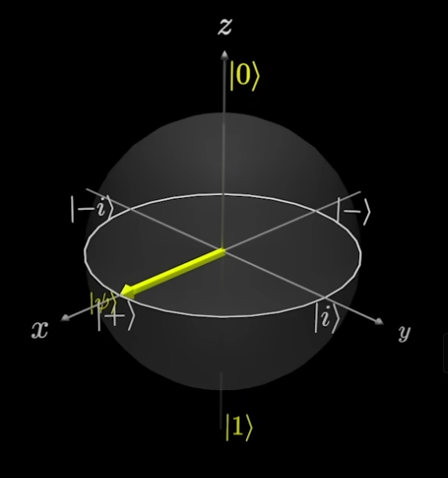
\includegraphics[width=5cm]{1}

Apparently, the `phase' around the z-axis that the qubit is pointed at is dependent only on the value of $\beta$. This is because we consider 2 types of phase: General phase, given by 

\[ 
    e^{i\phi}(\alpha \qb{0} + \beta \qb{1})
\]

and relative phase 

\[ 
    \alpha \qb{0} + e^{i\phi}\beta \qb{1}
\]

Apparently, general phase is something that is generally not really that important, and we want to consider relative phase in most cases. In general, if both $\qb{0}$ and $\qb{1}$ have some phase associated with it, we can factorise out one of them as a global phase, and `discard' it, leaving us with just the relative phase of one of $\qb{0}$ or $\qb{1}$

We now consider the X, Y, Z gates. They are defined as: 

\[
X = \begin{pmatrix} 0 & 1 \\ 1 & 0 \end{pmatrix} 
\quad 
Y = \begin{pmatrix} 0 & -i \\ i & 0 \end{pmatrix} 
\quad 
Z = \begin{pmatrix} 1 & 0 \\ 0 & -1 \end{pmatrix}
\]

\subsection*{3.2 Hadamard Gate}

We further note the existance of the H gate: 

\[
    H = \frac{1}{\sqrt{2}} \begin{pmatrix} 1 & 1 \\ 1 & -1 \end{pmatrix}
\]

The effect of this gate on $\qb{1}$ is to transform it to $\qb{-}$ and for $\qb{0}$ to  $\qb{+}$. 

\subsection*{3.3 S and T gates}

We note the following gates: 

\[
    S = \begin{pmatrix} 1 & 0 \\ 0 & e^{i \left(\frac{\pi}{2}\right)} \end{pmatrix}
\]

\[
    T = \begin{pmatrix} 1 & 0 \\ 0 & e^{i \left(\frac{\pi}{4}\right)} \end{pmatrix}
\]

The adjoint matrix of these 2 gates are its inverse, and their effect is to add a relative phase of 90 and 45 degrees respectively

\subsection*{3.4 Representing multiple qubits, and operations}

We represent qubits by their tensor product. In other words, we represent the 2 qubits: 

\[ 
    \qb{00} = \qb{0} \otimes \qb{0}
\]


This can be done for any number of qubits. When given 2 arbitary qubits that are tensor product-ed together, we can expand and write it in the general form. For instance, 

\[
\alpha\qb{00} + \alpha'\qb{01} + \beta\qb{10} + \beta'\qb{11}
\]

Furthermore, we can represent our manipulations to qubits as follows: 

\begin{center}
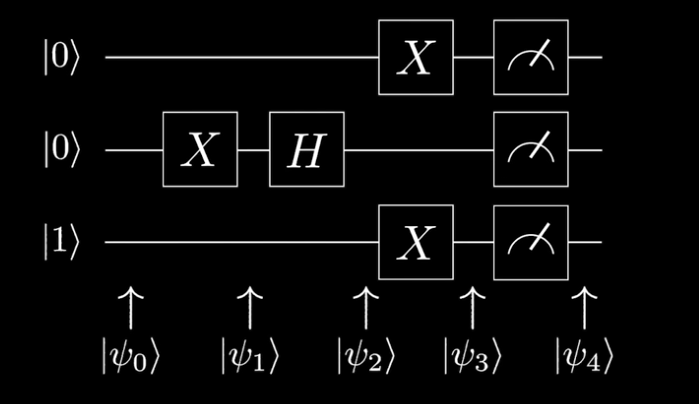
\includegraphics[width=5cm]{2}
\end{center}

In this case, we will be able to see that the final state is given by: 

\[ 
    \psi_3 = \frac{1}{\sqrt{2}} \left( \qb{100} - \qb{110} \right)
\]

so we see that the final state is either of the 2 above states, and measuring the qubits will result in the qubit collapsing into one of the 2 states. 

\subsection*{3.5 CNOT, Toffoli}

CNOT gates takes one gate as input and manipulates another gate. It applies an X gate to the target qubit if the control qubit is 1, and does nothing otherwise. 

\begin{center}
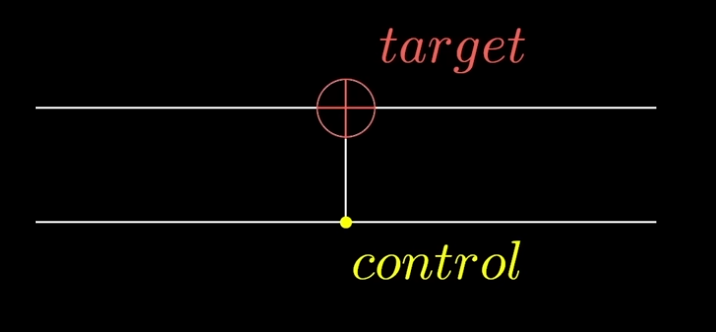
\includegraphics[width=5cm]{3}

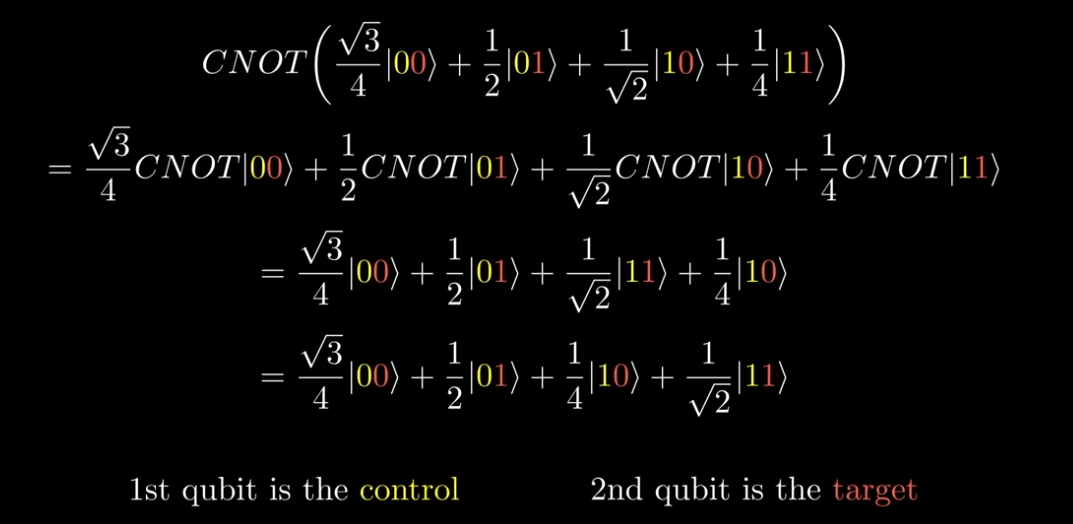
\includegraphics[width=11cm]{4}
\end{center}

Toffoli Gates operate with 2 control (read input) gates, and 1 target, rather than just 1 control, and require both control bits to be 1 to apply an X-gate to the target qubit.

We can further generalise this to the other existingly known gates; we can have controlled Y, Z, S, T and H gates, giving us some level of conditional logic to be applied. 

\begin{center}
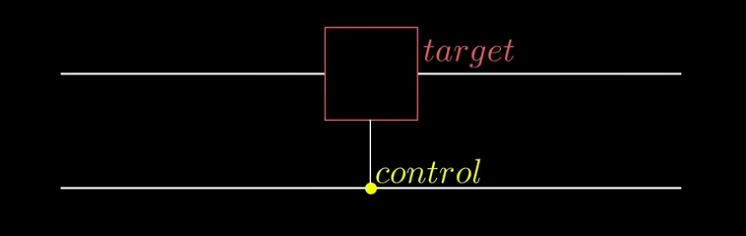
\includegraphics[width=5cm]{5}
\end{center}

We represent this in general as seen above. 

\subsection*{3.6 Measuring singular qubits}

In general, with multiple qubits that are manipulated, the probability of a singular qubit being something in the sum of squares of probabilities of that qubit being the stated value (with all other possible combination of other qubits.)

When we actually measure a given qubit, the state collapses, and we need to normalise the probabilities (just do the obvious, multiple all probabilities by a normalisation constant, and make sure this satisfies that the total probability is 1).

\section*{4 Quantum Mechanics}

\subsection*{4.1 Entanglement}

A state is entangled if it cannot be factored into the tensor product of individual qubits. In other words, qubits depend on each other, and measuring one will determine the others.

Maximally entanglement: If measurement of one of the qubit determines the state of the other qubits

Partially entangled: Measuring one of the qubits affects the amplitudes of the other qubits (i.e. measuring one changes the probability of the other). 

Bell states: 

\[
\begin{aligned}
|\Phi^+ \rangle &= \frac{1}{\sqrt{2}} \left( |00\rangle + |11\rangle \right) \\
|\Phi^- \rangle &= \frac{1}{\sqrt{2}} \left( |00\rangle - |11\rangle \right) \\
|\Psi^+ \rangle &= \frac{1}{\sqrt{2}} \left( |01\rangle + |10\rangle \right) \\
|\Psi^- \rangle &= \frac{1}{\sqrt{2}} \left( |01\rangle - |10\rangle \right)
\end{aligned}
\]

\subsection*{4.2 Phase Kickback}

In some control circumstances, the control qubit might be affected rather than the target qubit. This seems to happen in the case where the target qubit is a eigenvector of the gate. 

\begin{center}
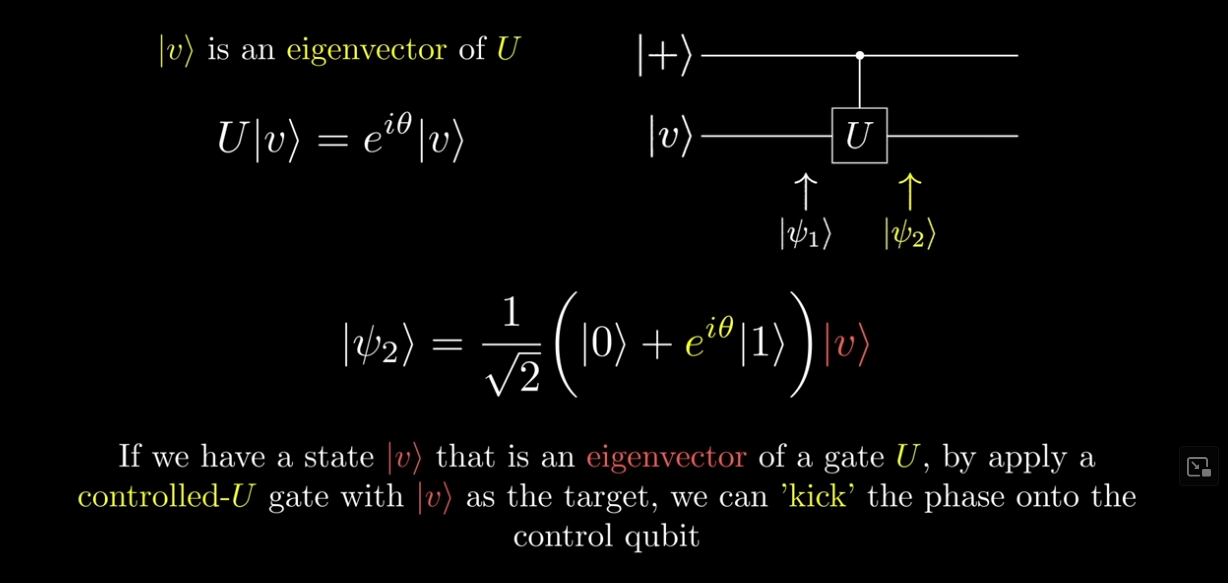
\includegraphics[width=10cm]{6}
\end{center}

\subsection*{4.3 A simple quantum algorithm}

Suppose we want to send 2 bits of information by sending on bit. One might do this by entangling 2 states first. If we each take 1 bit, I can perform operations on one qubit, and send it to you. Then, you might be able to perform a step of operations, to get the message I am trying to send. 

\begin{center}
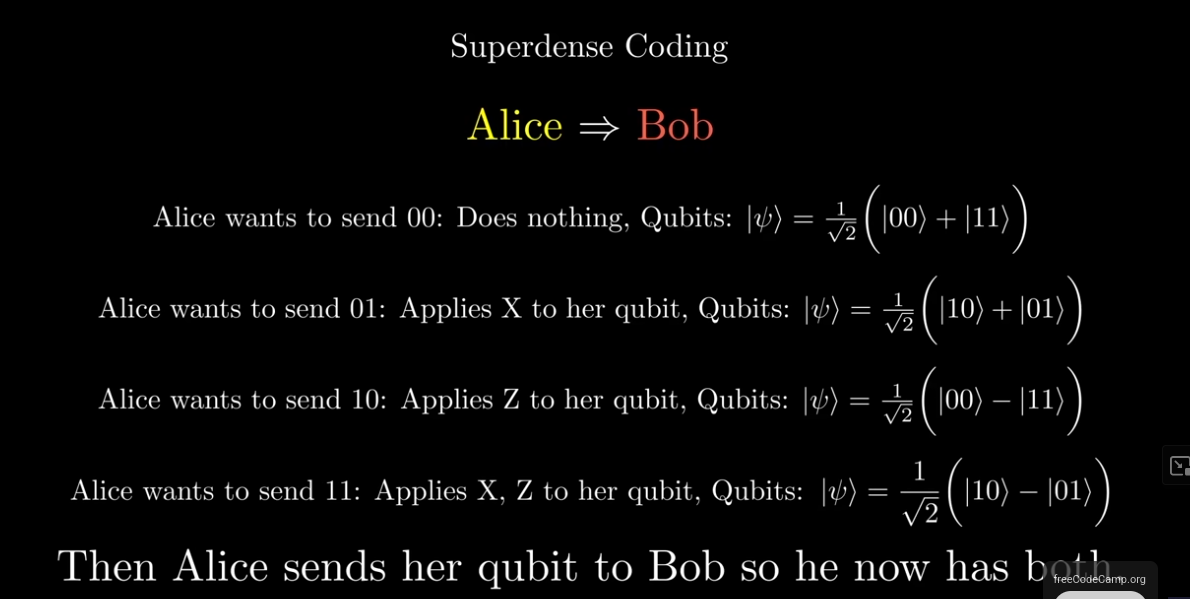
\includegraphics[width=10cm]{7}
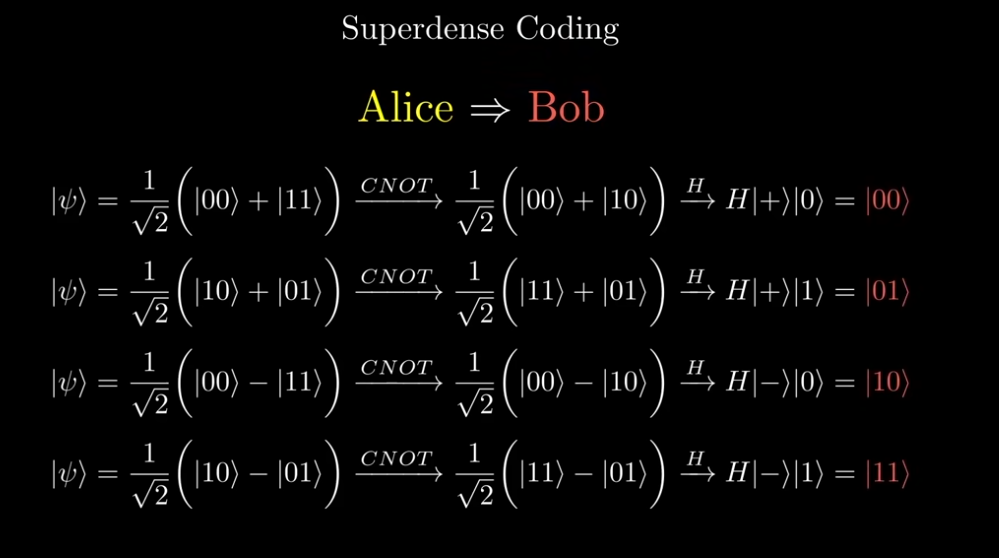
\includegraphics[width=10cm]{8}
\end{center}

\subsection*{4.4 Functions on Quantum Computers}

In general for our classical operations, they are not reversible. In other words, when performing the operation, we usually cannot obtain the input information from just the output information. We often need more information. 

One way that we can help this is by having some control bit $c$, which we XOR with the output of the function $f$. If we do this with 0, this just returns our output $f(x)$, and if we also output our input bits, we know for certain what our input was. 

\begin{center}
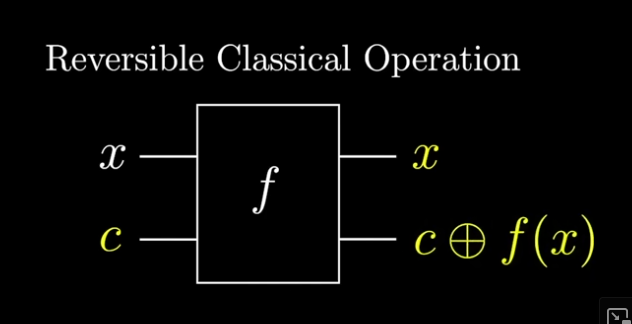
\includegraphics[width=10cm]{9}
\end{center}

We can employ such a strategy to the quantum functions, which as earlier stated due to the unitary nature of the functions, must be reversible. We want to input as the control qubit as $\qb{0}$ so we just get $f(x)$ out. 


\begin{center}
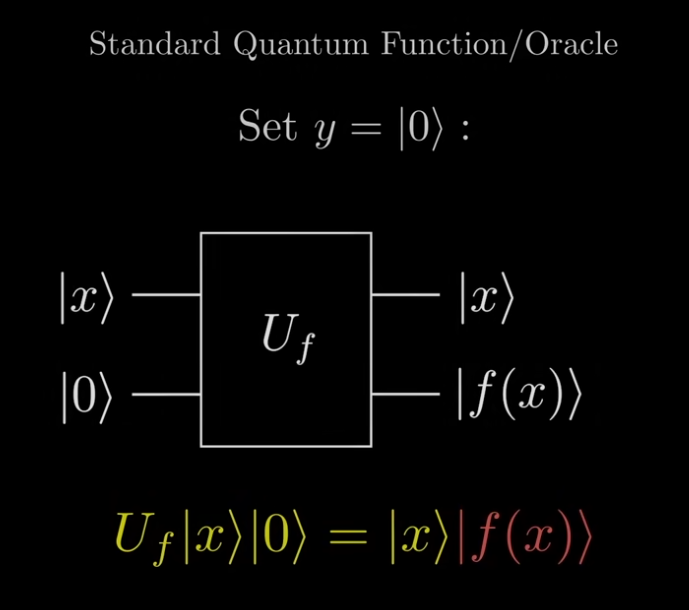
\includegraphics[width=10cm]{10}
\end{center}

Another special case we might note is if we had instead input the output bit as $\qb{-}$ instead. Our outputs will consist of our input $\qb{x}$ having a phase change, known as a phase oracle. 

\begin{center}
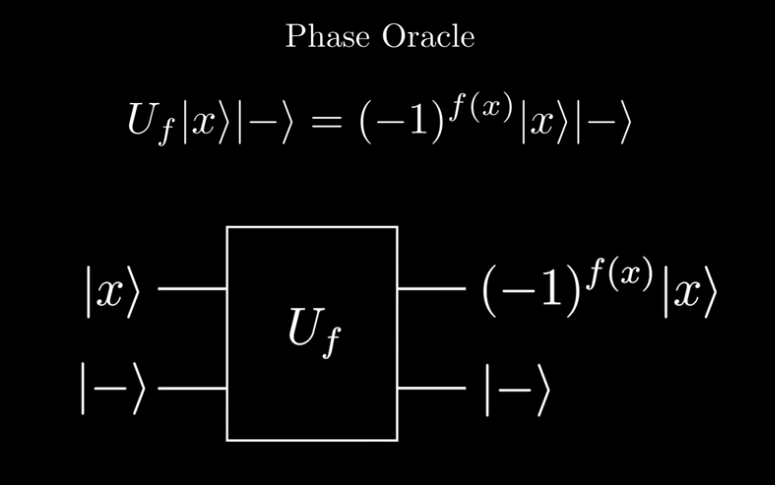
\includegraphics[width=10cm]{11}
\end{center}

\subsection*{4.5 Deutsch's Algorithm}

This algorithm serves to determine if a function is a constant function (in this case, alternative is a `balanced' function). In classical computers, we have to use 2 inputs, to compare them, but quantum computers allow us to do this once only. 

\begin{center}
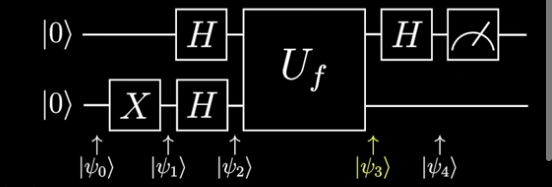
\includegraphics[width=10cm]{12}
\end{center}

This can be generalised with this other algorithm: 

\begin{center}
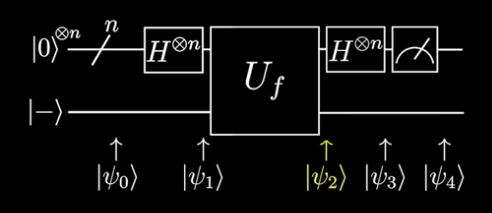
\includegraphics[width=10cm]{13}
\end{center}

This pattern of applying the H gate, then the function, and the H gate again seems to be a common theme in alot of algorithms.

What turns out to be really important in these calculations is these 2 identities. In other words, how to apply the H gate to some arbitrary bit string (read: some number of qubits)

\begin{center}
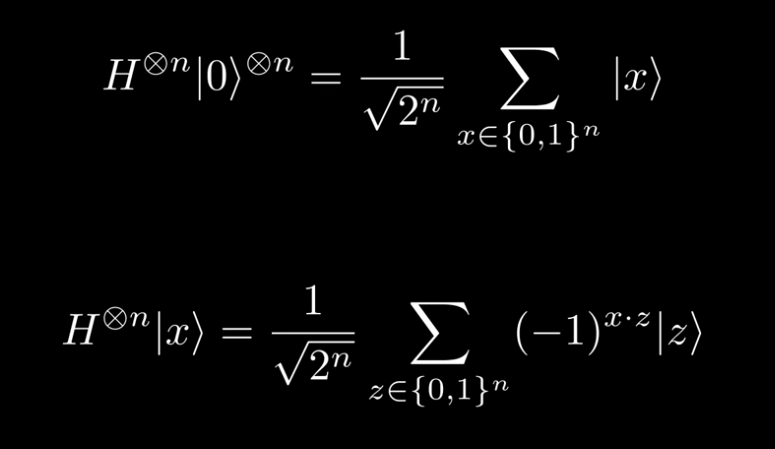
\includegraphics[width=10cm]{14}
\end{center}


\end{document}

